\documentclass{article}
\usepackage{tikz}
\usetikzlibrary{arrows.meta,positioning,calc,shapes.geometric}
\pagestyle{empty}
\begin{document}
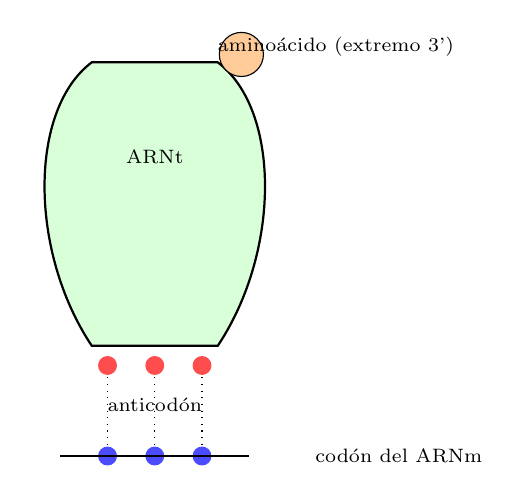
\begin{tikzpicture}

\draw[thick, fill=green!15] (0,0) .. controls (-0.8,1.2) and (-0.8,3.0) .. (0,3.6) -- (1.6,3.6) .. controls (2.4,3.0) and (2.4,1.2) .. (1.6,0) -- cycle;
\node[font=\scriptsize, align=center] at (0.8,2.4) {ARNt};
\draw[fill=orange!40] (1.9,3.7) circle (0.28); \node[font=\scriptsize] at (3.1,3.8) {aminoácido (extremo 3')};
\foreach \x in {0.2,0.8,1.4} {\fill[red!70] (\x,-0.25) circle (0.12);}
\node[font=\scriptsize] at (0.8,-0.75) {anticodón};
\foreach \x in {0.2,0.8,1.4} {\fill[blue!70] (\x,-1.4) circle (0.12);} \draw[thick] (-0.4,-1.4) -- (2.0,-1.4);
\node[font=\scriptsize] at (3.9,-1.4) {codón del ARNm};
\foreach \x in {0.2,0.8,1.4} {\draw[dotted] (\x,-0.4) -- (\x,-1.25);}

\end{tikzpicture}
\end{document}
